\documentclass[german]{uebung}

\usepackage{uebung-meta}
\usepackage{enumitem}
\usepackage{amssymb}
\usepackage{multicol}
\usepackage{listings}
\usepackage{hyperref}
\usepackage{appendix}


\lstset{language=python}
%%%%%%%%%%%%%%%%%%%%%%%%%%%%%%%%%%%%%%%%%%%%%%%%%%%%%%%%%%%%%%%%%%%%%%%%%%%%
% README
%%%%%%%%%%%%%%%%%%%%%%%%%%%%%%%%%%%%%%%%%%%%%%%%%%%%%%%%%%%%%%%%%%%%%%%%%%%%

% How to use this:
% 1. Add your data to uebung-meta.sty (you only need to do this once)
% 2. Copy this file and name it something useful
% 3. Set the assignment to the right value
% 4. Use the exercise enviroment to separate your solutions for the different exercises from each other.

% DO NOT CHANGE uebung.cls! If you need more packages just add a new \usepackage somewhere in this file before the \begin{document}

% The commands
% \div and \grad are provided by uebung.cls

% The environment "exercise" takes one parameter (the exercise number). 
% This way you can skip exercises if you like. Example:
% 
% \assignment{3}
% \begin{exercise}{8}
% ...
% \end{exercise}
% 
% The solution to exercise 3.8 (3rd assignment, 8th exercise) goes where 
% the dots are.

% If the total page number shows up as ?? in the footer you need to compile a second time.

% Which assignment is this?
\assignment{2}


\begin{document}

\begin{exercise}{1}
	\begin{enumerate}[label=(\alph*)]
		\item a
	Der Massenzufluss an Salz in das Gef\"a{\ss} pro Zeiteinheit sei definiert als $m_{in} = rc_0$.
	Weiterhin sei der Massenabflu{\ss} an Salz definiert als $m_{out} = rc$, mit $c = c(t)$.
	Die Menge an Salz im Gef\"a{\ss} definiert als $m = Vc$, mit $m = m(t)$, woraus sich eine
	zeitliche {\"A}nderung der Salzmasse im Gef\"a{\ss} von $\dot{m} = V\dot{c}$ ergibt.
	Diese l\"asst sich au{\ss}erdem darstellen als $m\dot = rc_0 - rc$.\\
	Kombiniert man diese Gleichungen, so erh\"alt man:

		\begin{alignat}{3}
			& \dot{m}	&&= \dot{m}	\\
			\leftrightarrow && V\dot{c}&= rc_0 - rc	\\
			\leftrightarrow	&& \dot{c} &= \frac{rc_0}{V} - \frac{rc}{V}
		\end{alignat}

		\item b
	\end{enumerate}
\end{exercise}

\begin{exercise}{2}
	L\"osungscode ist in der Angef\"ugten .ipynb Datei und im \hyperref[lab:ap]{Appendix}
	des PDFs angegeben. Ein direkter Link befindet sich im jeweiligen
	Aufgabenteil. Die berechneten L\"oesungspunkte wurden mittels Jupyter
	Notebook bestimmt (Ergebnisse zu finden \"ueber dem Plot).
	\begin{enumerate}[label=(\alph*)]
		\item \hyperref[codeA]{L\"osungscode expliziter Euler}\\
			Berechnete L\"osungspunkte f\"ur $t = 0, 1, 2$: 1.0, 1.33333333, 1.63665777
		\item \hyperref[codeB]{L\"osungscode impliziter Euler}\\
			Berechnete L\"osungspunkte f\"ur $t = 0, 1, 2$: 1.0, 1.28831999, 2.35160323
		\item \hyperref[codeC]{L\"osungscode Heun}\\
			Berechnete L\"osungspunkte f\"ur $t = 0, 1, 2$: 1.0, 1.31832888, 1.87664008
		\item \hyperref[codeD]{L\"osungscode Runge-Kutta}\\
			Berechnete L\"osungspunkte f\"ur $t = 0, 1, 2$: 1.0, 0.58699063, 1.60222733
	\end{enumerate}

	\hyperref[fig:1]{Figure 1} zeigt das Ergebnis der Berechnungen als Plot dargestellt.
	\begin{figure}[h]
		\centering
		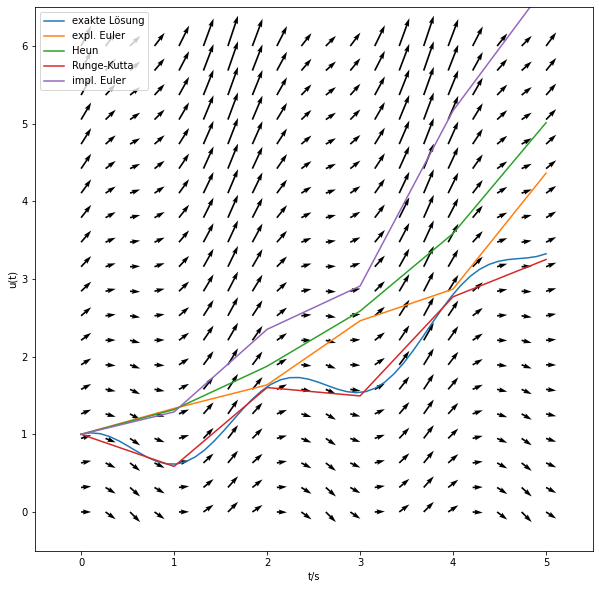
\includegraphics[width=0.6\textwidth]{plot.png}
		\caption{Ergebnisse aller Einschrittverfahren geplottet gegen
			die exakte L\"osung}
		\label{fig:1}
	\end{figure}
\end{exercise}

\begin{exercise}{3}
	\begin{enumerate}[label=(\alph*)]
		\item $a$ und $b$ sind \"Uebergangsvariablen, die die \"Anderungrate
			der Susceptibles zu Infected ($a$), bzw. die \"Anderungrate
			von Infected zu Recovered ($b$) pro Zeiteinheit modellieren.
			Hierbei stehen $a$ und $b$ allerdings nicht nur f\"ur eine
			'simple' Infektions-, bzw. Genesungsrate, sondern schlie{\ss}en
			alle m\"oglichen Faktoren ein, die zum Infektions-/Genesungsgeschehen
			beitragen.
		\item Der komplette Code zur L\"osung ist im beigef\"ugten Jupyter Notebook einsehbar.
			Das Modell selbst war definiert durch den unten stehenden Code. Die Zeitabh\"angigkeit
			der einzelnen Variablen wird implizit \"uber ihre Position in
			der L\"osungsliste miteinbezogen. $V(t)$ und $c$ wurden aus
			Einfachheit bereits nonfunktional miteinbezogen. Als Einschrittverfahren
			wurde das explizite Euler-Verfahren gew\"ahlt.

			\begin{lstlisting}[frame=single]
def SUS(SIRV, a=0.5, b=0.1):
    return -a*SIRV[0]*SIRV[1]

def INF(SIRV, a=0.5, b=0.1):
    return a*SIRV[0]*SIRV[1] - b*SIRV[1]

def REC(SIRV, a=0.5, b=0.1):
    return b*SIRV[1]

def VAC(SIRV, a=0.5, b=0.1):
    return 0
			\end{lstlisting}

			Folgend das Ergebnis der Berechnung in \hyperref[fig:p2]{Figure 2}:
			\begin{figure}[h!]
				\centering
				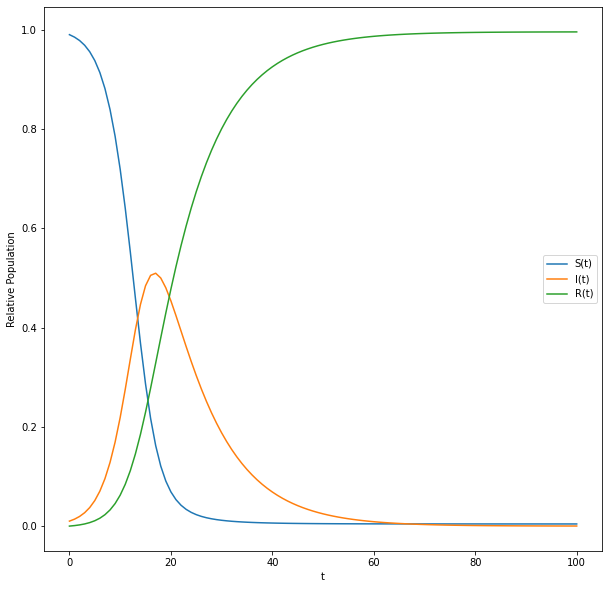
\includegraphics[width=0.5\textwidth]{plot2.png}
				\caption{L\"osung des SIR-Modells mittels explizitem Euler-Verfahren}
				\label{fig:p2}
			\end{figure}
		\item \begin{align}
				\frac{dS}{dt} &= -aS(t)I(t) - cS(t)\\
				\frac{dI}{dt} &= aS(t)I(t) - bI(t) - cI(t)\\
				\frac{dR}{dt} &= bI(t) - cR(t)\\
				\frac{dV}{dt} &= cS(t) + cI(t) + cR(t)
			\end{align}

		\item Das erweitere Modell wurde mit dem analogen Code simuliert der auch in (b) verwendet wurde.
			Allerdings wurden die Funktionen f\"ur die einzelnen Gruppen entsprechend (c) angepasst. Der
			Code ist im Folgenden zu sehen.
			
			\begin{lstlisting}[frame=single]
def SUS(SIRV, a=0.5, b=0.1, c=0.01):
    return -a*SIRV[0]*SIRV[1] - c*SIRV[0]

def INF(SIRV, a=0.5, b=0.1, c=0.01):
    return a*SIRV[0]*SIRV[1] - b*SIRV[1] - c*SIRV[1]

def REC(SIRV, a=0.5, b=0.1, c=0.01):
    return b*SIRV[1] - c*SIRV[2]

def VAC(SIRV, a=0.5, b=0.1, c=0.01):
    return c*SIRV[0] + c*SIRV[1] + c*SIRV[2]
			\end{lstlisting}
			
			Folgend das Ergebnis der Berechnung in \hyperref[fig:p3]{Figure 3}:
			\begin{figure}[h!]
				\centering
				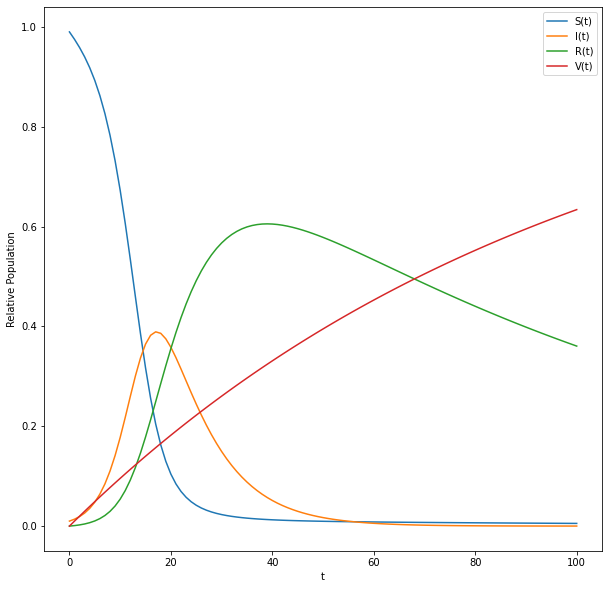
\includegraphics[width=0.5\textwidth]{plot3.png}
				\caption{L\"osung des erweiterten SIR-Modells mittels explizitem Euler-Verfahren}
				\label{fig:p3}
			\end{figure}

	\end{enumerate}
\end{exercise}
\;\newpage

\section*{Appendix}\label{lab:ap}
\label{codeA}Code f\"ur explizites Euler-Verfahren:
\begin{lstlisting}[frame=single]
def explicit_euler(f, u0, t_disc):
    
    # neuer array mit u0 als erstem Element. Wenn u0 ein Vektor ist,
    # wird u so ein zweidimensionaler Array
    u = np.zeros((len(t_disc), len(u0))) #Loesungsmatrix
    u[0] = u0                            #Anfangswert
    
    for i in range(1, len(t_disc)):
        t_last = t_disc[i-1]
        t = t_disc[i]
        tau = t-t_last
        
        # der letzte berechnete Wert von u
        u_last = u[i-1]
        
        # Ausfuehrung des Zeitschritts
        u_new = u_last + tau*f(t_last, u_last)
                        
        # Speichern des neuen Werts
        u[i] = u_new
    
    return u
\end{lstlisting}
\;\newline
\label{codeB}Code f\"ur implizites Euler-Verfahren:
\begin{lstlisting}[frame=single]
def implizit_euler(f, u0, t_disc):
    u = np.zeros((len(t_disc), len(u0)))
    u[0] = u0
    
    for i in range(1, len(t_disc)):

        t_last=t_disc[i-1]
        t = t_disc[i]
        tau = t-t_last
        u_last = u[i-1]
        # bis hier analog zu euler
        
        # berechne ui anhand der im Notebook gegebenen Gleichung
        u[i] = (u_last + tau*-1*np.sin(3*t))/(1-(tau/3))
    return u
\end{lstlisting}
\newpage
\;\newline
\label{codeC}Code f\"ur Heun-Verfahren:
\begin{lstlisting}[frame=single]
def heun(f, u0, t_disc):
    
    u = np.zeros((len(t_disc), len(u0)))
    u[0] = u0
    
    for i in range(1, len(t_disc)):
        t_last=t_disc[i-1]
        t = t_disc[i]
        tau = t-t_last
        u_last = u[i-1]
        # bis hier analog zu euler
        
        #berechne k1 und k2
        k1 = f(t_last, u_last)
        k2 = f(t, u_last + tau*k1)
        
        #Kombiniere zu neuer Loesung
        u[i] = u_last + tau*(1/2)*(k1 + k2)
    return u
\end{lstlisting}
\;\newline
\label{codeD}Code f\"ur Runge-Kutta-Verfahren:
\begin{lstlisting}[frame=single]
def runge_kutta(f, u0, t_disc):
    
    u = np.zeros((len(t_disc), len(u0)))
    u[0] = u0
    
    for i in range(1, len(t_disc)):

        t_last=t_disc[i-1]
        t = t_disc[i]
        tau = t-t_last
        u_last = u[i-1]
        # bis hier analog zu euler
    
        #berechne k1,k2,k3 und k4
        tau_h = tau * (1/2)
        k1 = f(t_last, u_last)
        k2 = f(t_last + tau_h, u_last+tau_h*k1)
        k3 = f(t_last + tau_h, u_last+tau_h*k2)
        k4 = f(t, u_last+tau*k3)

        #Kombiniere zu neuer Loesung
        u[i] = u_last + tau*(1/6)*(k1+(2*k2)+(2*k3)+k4)
    return u
    
\end{lstlisting}

\end{document}
